\documentclass{beamer}
\usepackage[orientation=portrait, size=a0, scale=1.1]{beamerposter}
\usepackage{multicol} % This is so we can have multiple columns of text side-by-side
\usepackage{parskip}
%\usepackage{enumitem}
%\setlist[itemize]{parsep=0pt}
%\setlist[enumerate]{parsep=0pt}
%\parindent=0em

%% Bibliography stuff (biblatex):
\usepackage[
backend=bibtex,
firstinits=true, 
isbn=false, 
url=false,
maxbibnames=3,
doi=false,
clearlang=true,
terseinits=true,
citestyle=numeric,
autolang=hyphen,
clearlang=true
]{biblatex} 

\AtEveryBibitem{%
  \clearlist{language}%
}


\renewcommand*{\bibfont}{\small}
%\bibliography{library.bib}


\usetheme{BCCRC}

\title{Screw: tools for building reproducible single-cell epigenomics workflows}
\author{Kieran O'Neill, Chelsey Fang, Benjamin Decato, Azhar Khandekar, Alexander Goncearenco, Ben Busby, Aly Karsan}
\institute{Genome Sciences Centre, BC Cancer Agency, Vancouver, BC, Canada}


\begin{document}
\begin{frame}[t, squeeze, fragile]
\begin{columns}[t]

%%%%%%%%%%%%%%%%%%%%%%%%%%%%%%%%%%%%%%%%%%%%%%%%%%%%%%%%%%%%%%%%%%%%%%%%%%%%%%%%%%%%
% COLUMN 1
%%%%%%%%%%%%%%%%%%%%%%%%%%%%%%%%%%%%%%%%%%%%%%%%%%%%%%%%%%%%%%%%%%%%%%%%%%%%%%%%%%%%


\begin{column}{.32\textwidth}


\begin{block}{Background: Single-cell DNA Methylation Sequencing}
DNA methylation is a heritable epigenetic mark that shows a strong correlation with transcriptional activity. 
The gold standard for detecting DNA methylation is whole genome bisulfite sequencing (WGBS). 
Recently, WGBS has been performed successfully on single cells (SC-WGBS) [@Schwartzman2015].
The resulting data represents a fundamental shift in the capacity to measure and interpret DNA methylation, especially in rare cell types and contexts where subtle cell-to-cell heterogeneity is crucial, such as in stem cells or cancer. 

\begin{figure}
\begin{center}
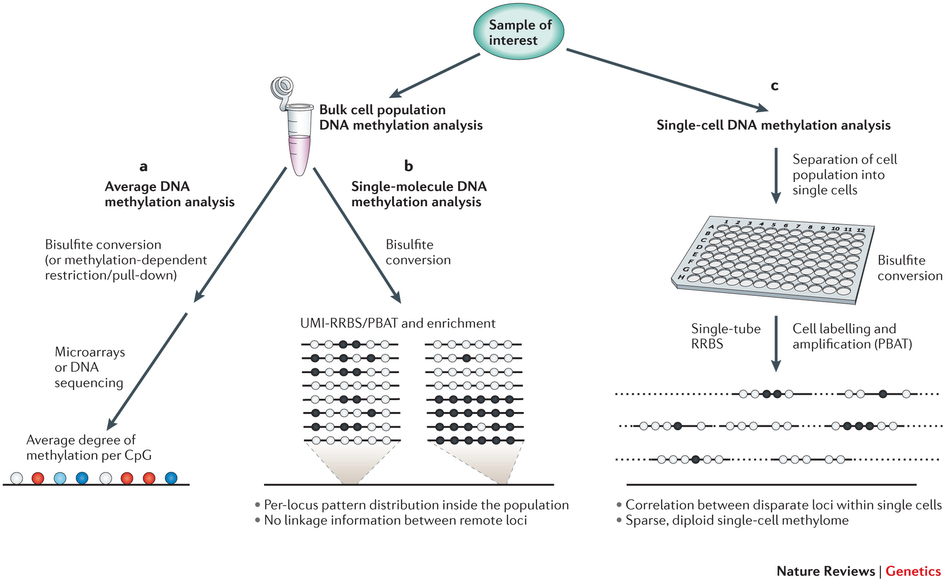
\includegraphics[width=0.9\textwidth]{figures/nrg3980-f1.jpg}
\end{center}
\caption[]{\textbf{DNA Methylation, both bulk and single cell}
\small{Schwartzman et al (2015) Nature Reviews in Genetics (used by permission) } }
\end{figure}

\end{block}


\begin{block}{Reproducible Research with CWL and Docker}
Reproducible research means completely reproducing a given bioinformatic analysis
This requires having the exact \textbf{data}, \textbf{code} and \textbf{software} that was used.

\begin{itemize}
\item Open data in bioinformatics is a fairly solved problem.
\item Code is getting there with RMarkdown/Jupyter, but could be better.
\item Software versions (and accompanying OS/ecosystem) are a big problem.
\end{itemize}
CWL aims to provide a uniform and fully reproducible way of representing bioinformatics workflows. Docker aims to provide the exact environment in which an analysis was run. Together, they promise to help bioinformaticians to publish fully reproducible research.

As a side effect, Dockstore enables easy sharing of workflow components to help build new workflows. 
\end{block}


\begin{block}{Enter Screw}
Screw stands for Single Cell Reproducible Epigenomics Workflow

Screw aims to provide a series of CWL+Dockerised mini-workflows and workflow components for creating fully reproducible single-cell DNA methylation analysis.
\end{block}


\begin{block}{What SC-WGBS Data Looks Like}
\begin{center}
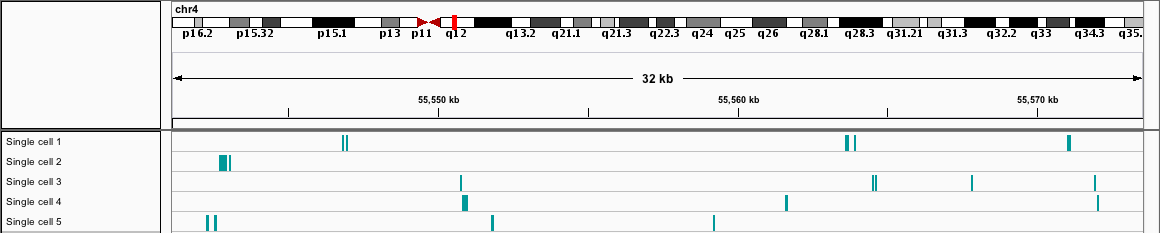
\includegraphics[width=0.9\textwidth]{figures/igv_sc.png}
\end{center}

\end{block}





\end{column}

%%%%%%%%%%%%%%%%%%%%%%%%%%%%%%%%%%%%%%%%%%%%%%%%%%%%%%%%%%%%%%%%%%%%%%%%%%%%%%%%%%%%
% COLUMN 2
%%%%%%%%%%%%%%%%%%%%%%%%%%%%%%%%%%%%%%%%%%%%%%%%%%%%%%%%%%%%%%%%%%%%%%%%%%%%%%%%%%%%

\begin{column}{.65\textwidth}
\vspace*{-\baselineskip}
  \begin{columns}[t,totalwidth=\textwidth]
    \begin{column}{.48\textwidth}
	%Second column, above figure
    
	\begin{block}{Preprocessing}
	
	\end{block}

	\end{column}

	\begin{column}{.48\textwidth}
	%Third column, above figure
	\begin{block}{Clustering}
	
	\end{block}

	\end{column}
  \end{columns}

	\begin{block}{Screw Workflow}
  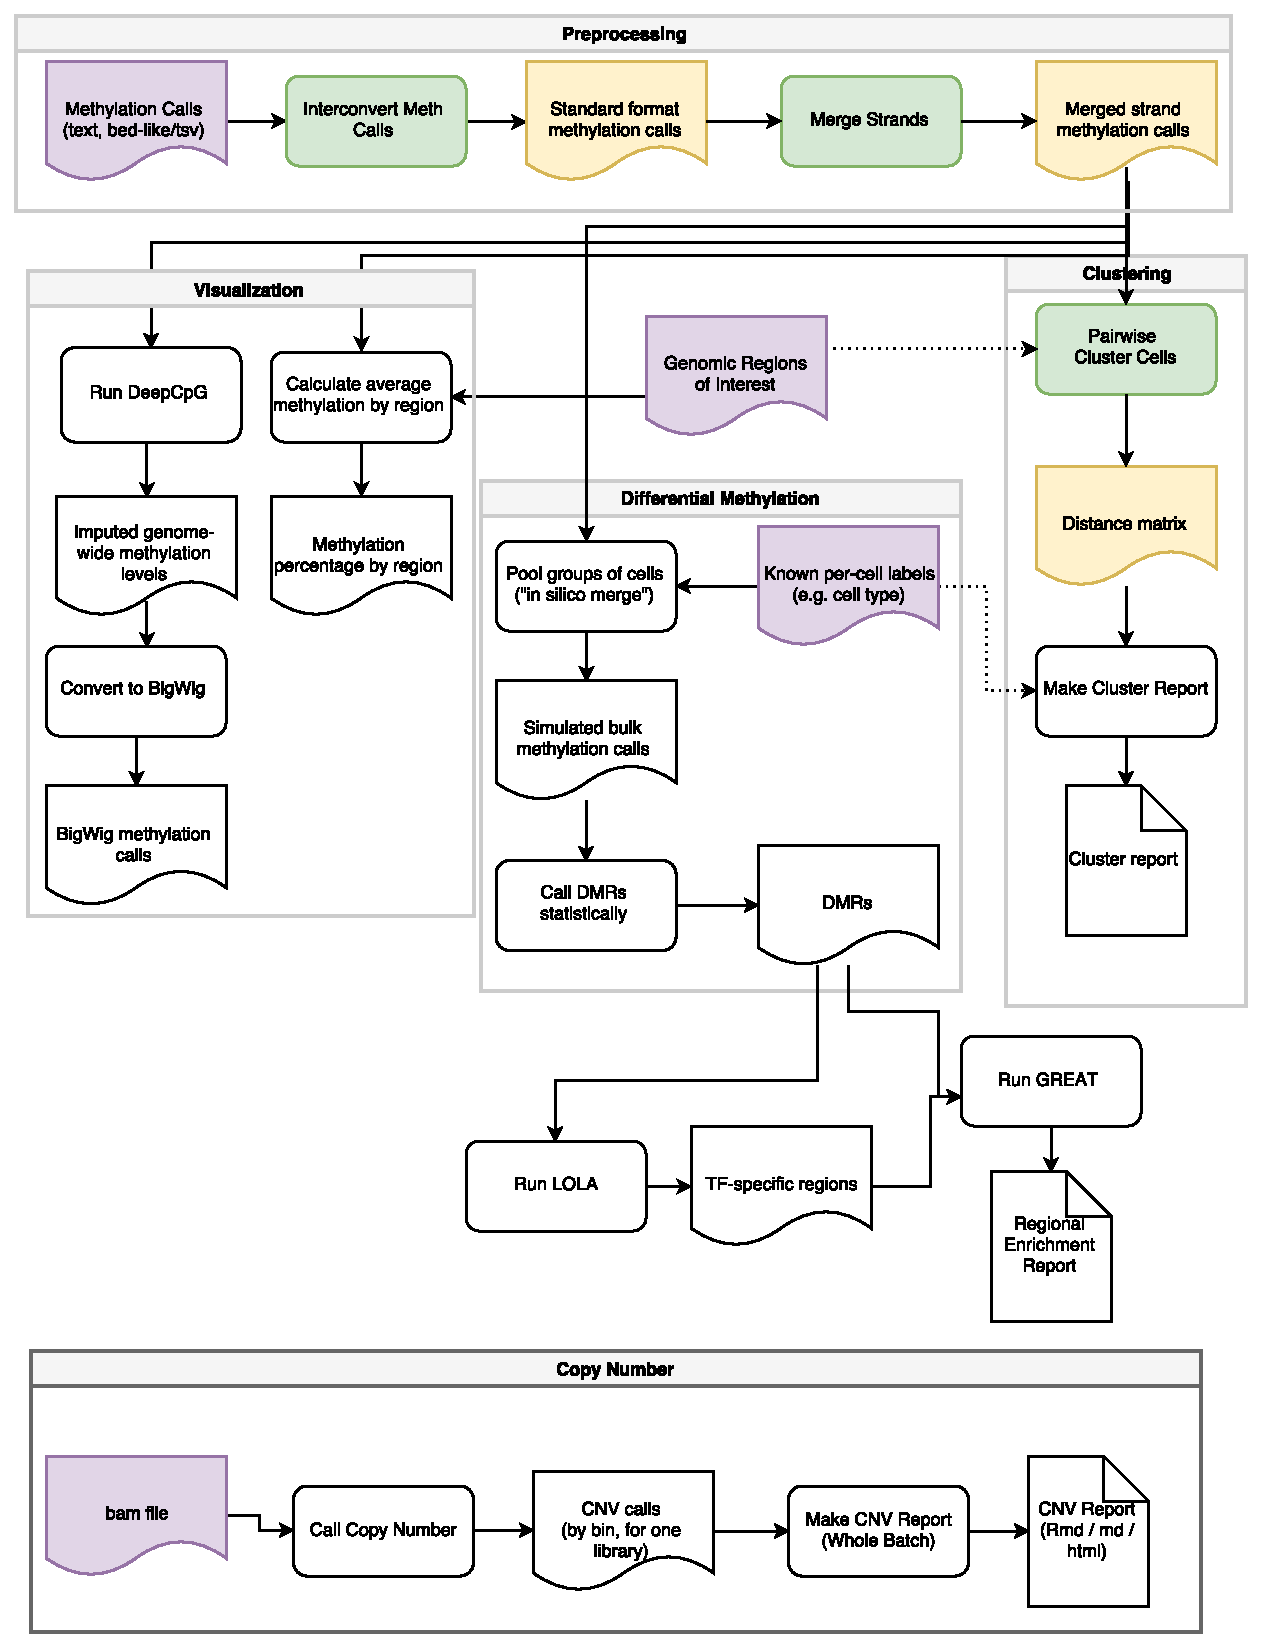
\includegraphics[width=\textwidth]{figures/workflow_diagram.pdf}
  \end{block}
  \begin{columns}[t,totalwidth=\textwidth]


\begin{column}{.48\textwidth}
   

% Second column, below figure   
    
\begin{block}{CWL Stumbling Blocks}

\end{block}



\begin{block}{Future Plans}

tSNE

\end{block}
\end{column}

	\begin{column}{.48\textwidth}
% Third column, below figure   
\begin{block}{How did Screw come about?}
Screw was initially created during the NCBI Genomics Hackathon in March 2017, organised by Ben Busby.
\begin{center}
  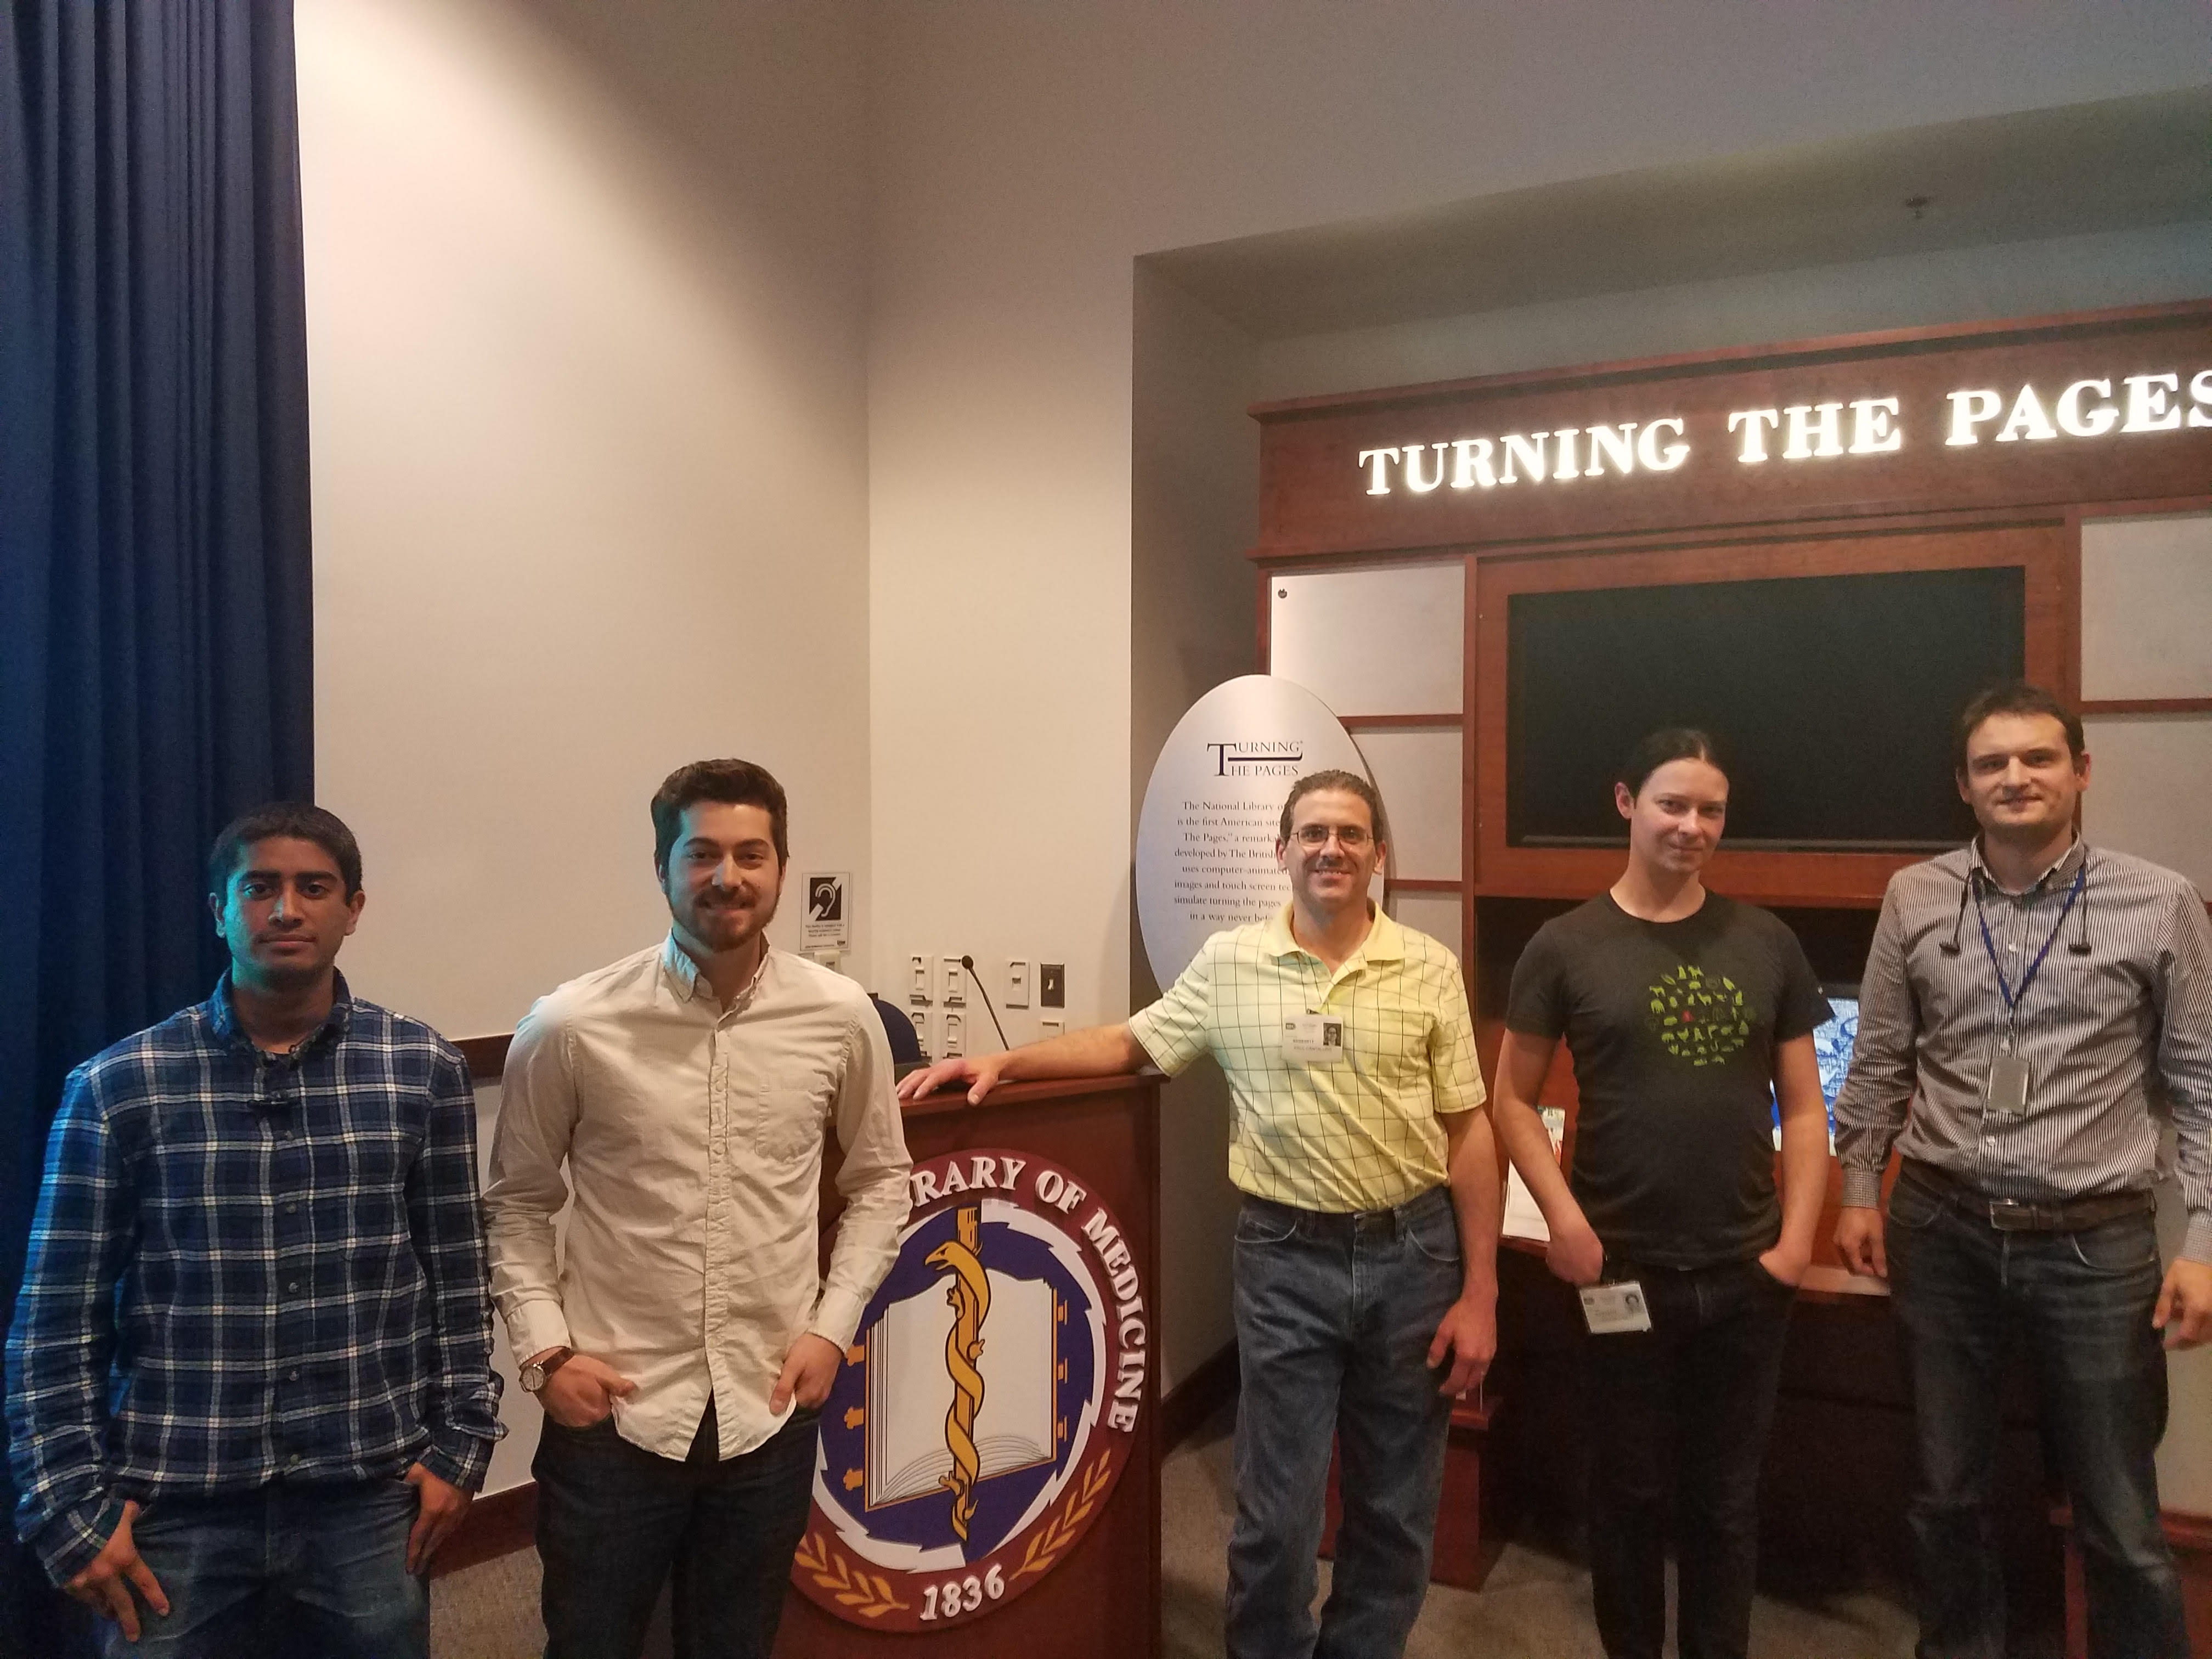
\includegraphics[width=\textwidth]{figures/hackathon_team.jpg}
\end{center}

\end{block}


\begin{block}{Contact/GitHub}
\textbf{GitHUB:} \verb1https://github.com/Epigenomics-Screw1  

\textbf{Kieran O'Neill:} koneill@bcgsc.ca 

\end{block}
 
\end{column}

  \end{columns}
\end{column}


\end{columns}

\end{frame}

\end{document}
